\documentclass[../../main.tex]{subfiles}

\graphicspath{{../../fig/}}
\setcounter{section}{0}

\begin{document}
\chapter{重力参照計の評価}
\label{chap:tiltsensor}
\ref{subsec:wg_tiltsensor}にて述べたように、本較正装置では重力参照計を用いて絶対角度を測定するが、
これまでに使用が想定されていた Digi-Pas 社製の DWL5000-XY は要求性能を満たさなかった。
今回、新たに候補となった Sherborne Sensors 社製の DSIC-2051-60 を評価した。
本章では、はじめに要求精度と評価すべき事項について確認したのち、本重力参照計の概要を共有、評価手法と結果について述べる。
\section{要求精度と評価内容}
要求される精度は、表\ref{tab:systematic_errors_old}中にある値から合計誤差が $\delta\theta < 0.1\tcdegree$ となることであり、
式\eqref{eq:wg_theta_sens}で表される $\theta_{\mathrm{sens}}$ にして $\delta\theta_{\mathrm{sens}}<0.06\tcdegree$ である。
これを重力参照計の要求精度に換算する。
式\eqref{}より、重力参照計の各 $X$ 軸、$Y$ 軸の誤差を $\delta\theta_{X},\,\delta\theta_{Y}$ とすると、
$\theta_{\mathrm{sens}}$ の誤差 $\delta\theta_{\mathrm{sens}}$ は
\begin{align}
    \delta\theta_{\mathrm{sens}} &= 
        \sqrt{\qty(\dfrac{\sin\beta}{\sin^2\alpha+\sin^2\beta} \delta\qty(\sin\alpha))^2 + \qty(\dfrac{\sin\alpha}{\sin^2\alpha+\sin^2\beta} \delta\qty(\sin\beta))^2}\\ 
    \delta\qty(\sin\alpha) &= \sqrt{\qty(\dv{\sin\alpha}{\theta_X}\delta\theta_X)^2+\qty(\dv{\sin\alpha}{\theta_Y}\delta\theta_Y)^2}\\
    \delta\qty(\sin\beta) &= \sqrt{\qty(\dv{\sin\beta}{\theta_X}\delta\theta_X)^2+\qty(\dv{\sin\beta}{\theta_Y}\delta\theta_Y)^2} \\
    \dv{\sin\alpha}{\theta_X} &= \cos\theta_{\mathrm{slope}1}\cos\theta_X - \sin\theta_{\mathrm{slope}1}\sin\theta_{\mathrm{slope}2}\dfrac{\sin\theta_X\cos\theta_X}{\sqrt{1-\sin^2\theta_X-\sin^2\theta_Y}} \\
    \dv{\sin\alpha}{\theta_Y} &= -\sin\theta_{\mathrm{slope}1}\cos\theta_{\mathrm{slope}2}\cos\theta_Y - \sin\theta_{\mathrm{slope}1}\sin\theta_{\mathrm{slope}2}\dfrac{\sin\theta_Y\cos\theta_Y}{\sqrt{1-\sin^2\theta_X-\sin^2\theta_Y}} \\
    \dv{\sin\beta}{\theta_X} &= \sin\theta_{\mathrm{slope}1}\cos\theta_X + \cos\theta_{\mathrm{slope}1}\sin\theta_{\mathrm{slope}2}\dfrac{\sin\theta_X\cos\theta_X}{\sqrt{1-\sin^2\theta_X-\sin^2\theta_Y}} \\
    \dv{\sin\beta}{\theta_Y} &= \cos\theta_{\mathrm{slope}1}\cos\theta_{\mathrm{slope}2}\cos\theta_Y + \cos\theta_{\mathrm{slope}1}\sin\theta_{\mathrm{slope}2}\dfrac{\sin\theta_Y\cos\theta_Y}{\sqrt{1-\sin^2\theta_X-\sin^2\theta_Y}}
\end{align}
のように表される。
$\theta_{\mathrm{slope}1}=210\tcdegree,\,\theta_{\mathrm{slope}2}=40\tcdegree$ は\ref{subsubsec:wg_tiltsensor_slope}にて導入したスロープの角度である。
重力参照計の両軸ともに同程度の誤差を持つと仮定し、スロープの角度から生じる誤差を無視すると、およそ $\delta\theta_{X} \sim \delta\theta_{Y} \leq 0.04\tcdegree$ が要求精度となる。

観測サイトはその気温が $\SI{-15}{\degreeCelsius} \sim \SI{20}{\degreeCelsius}$ と変動する過酷な環境である。
そのため、恒温槽を用いてこの温度の下で出力結果を測定し、温度変動による出力の変動を評価を行う。

\section{重力参照計の概要}
図\ref{fig:tiltsensor_DSIC-2051-60}に本重力参照計の外観を示す。
図中の $X$ 軸、$Y$ 軸と重力に対して垂直に交わる水平面のなす角が $\theta_{X},\,\theta_{Y}$ であり、これを出力する。
また、各軸は対応するセンサの温度も出力することができる。
公称の精度は $0.08\tcdegree$ であるため、その精度を再評価し、要求精度を満たすかを確認する必要がある。
\begin{figure}[H]
    \centering
    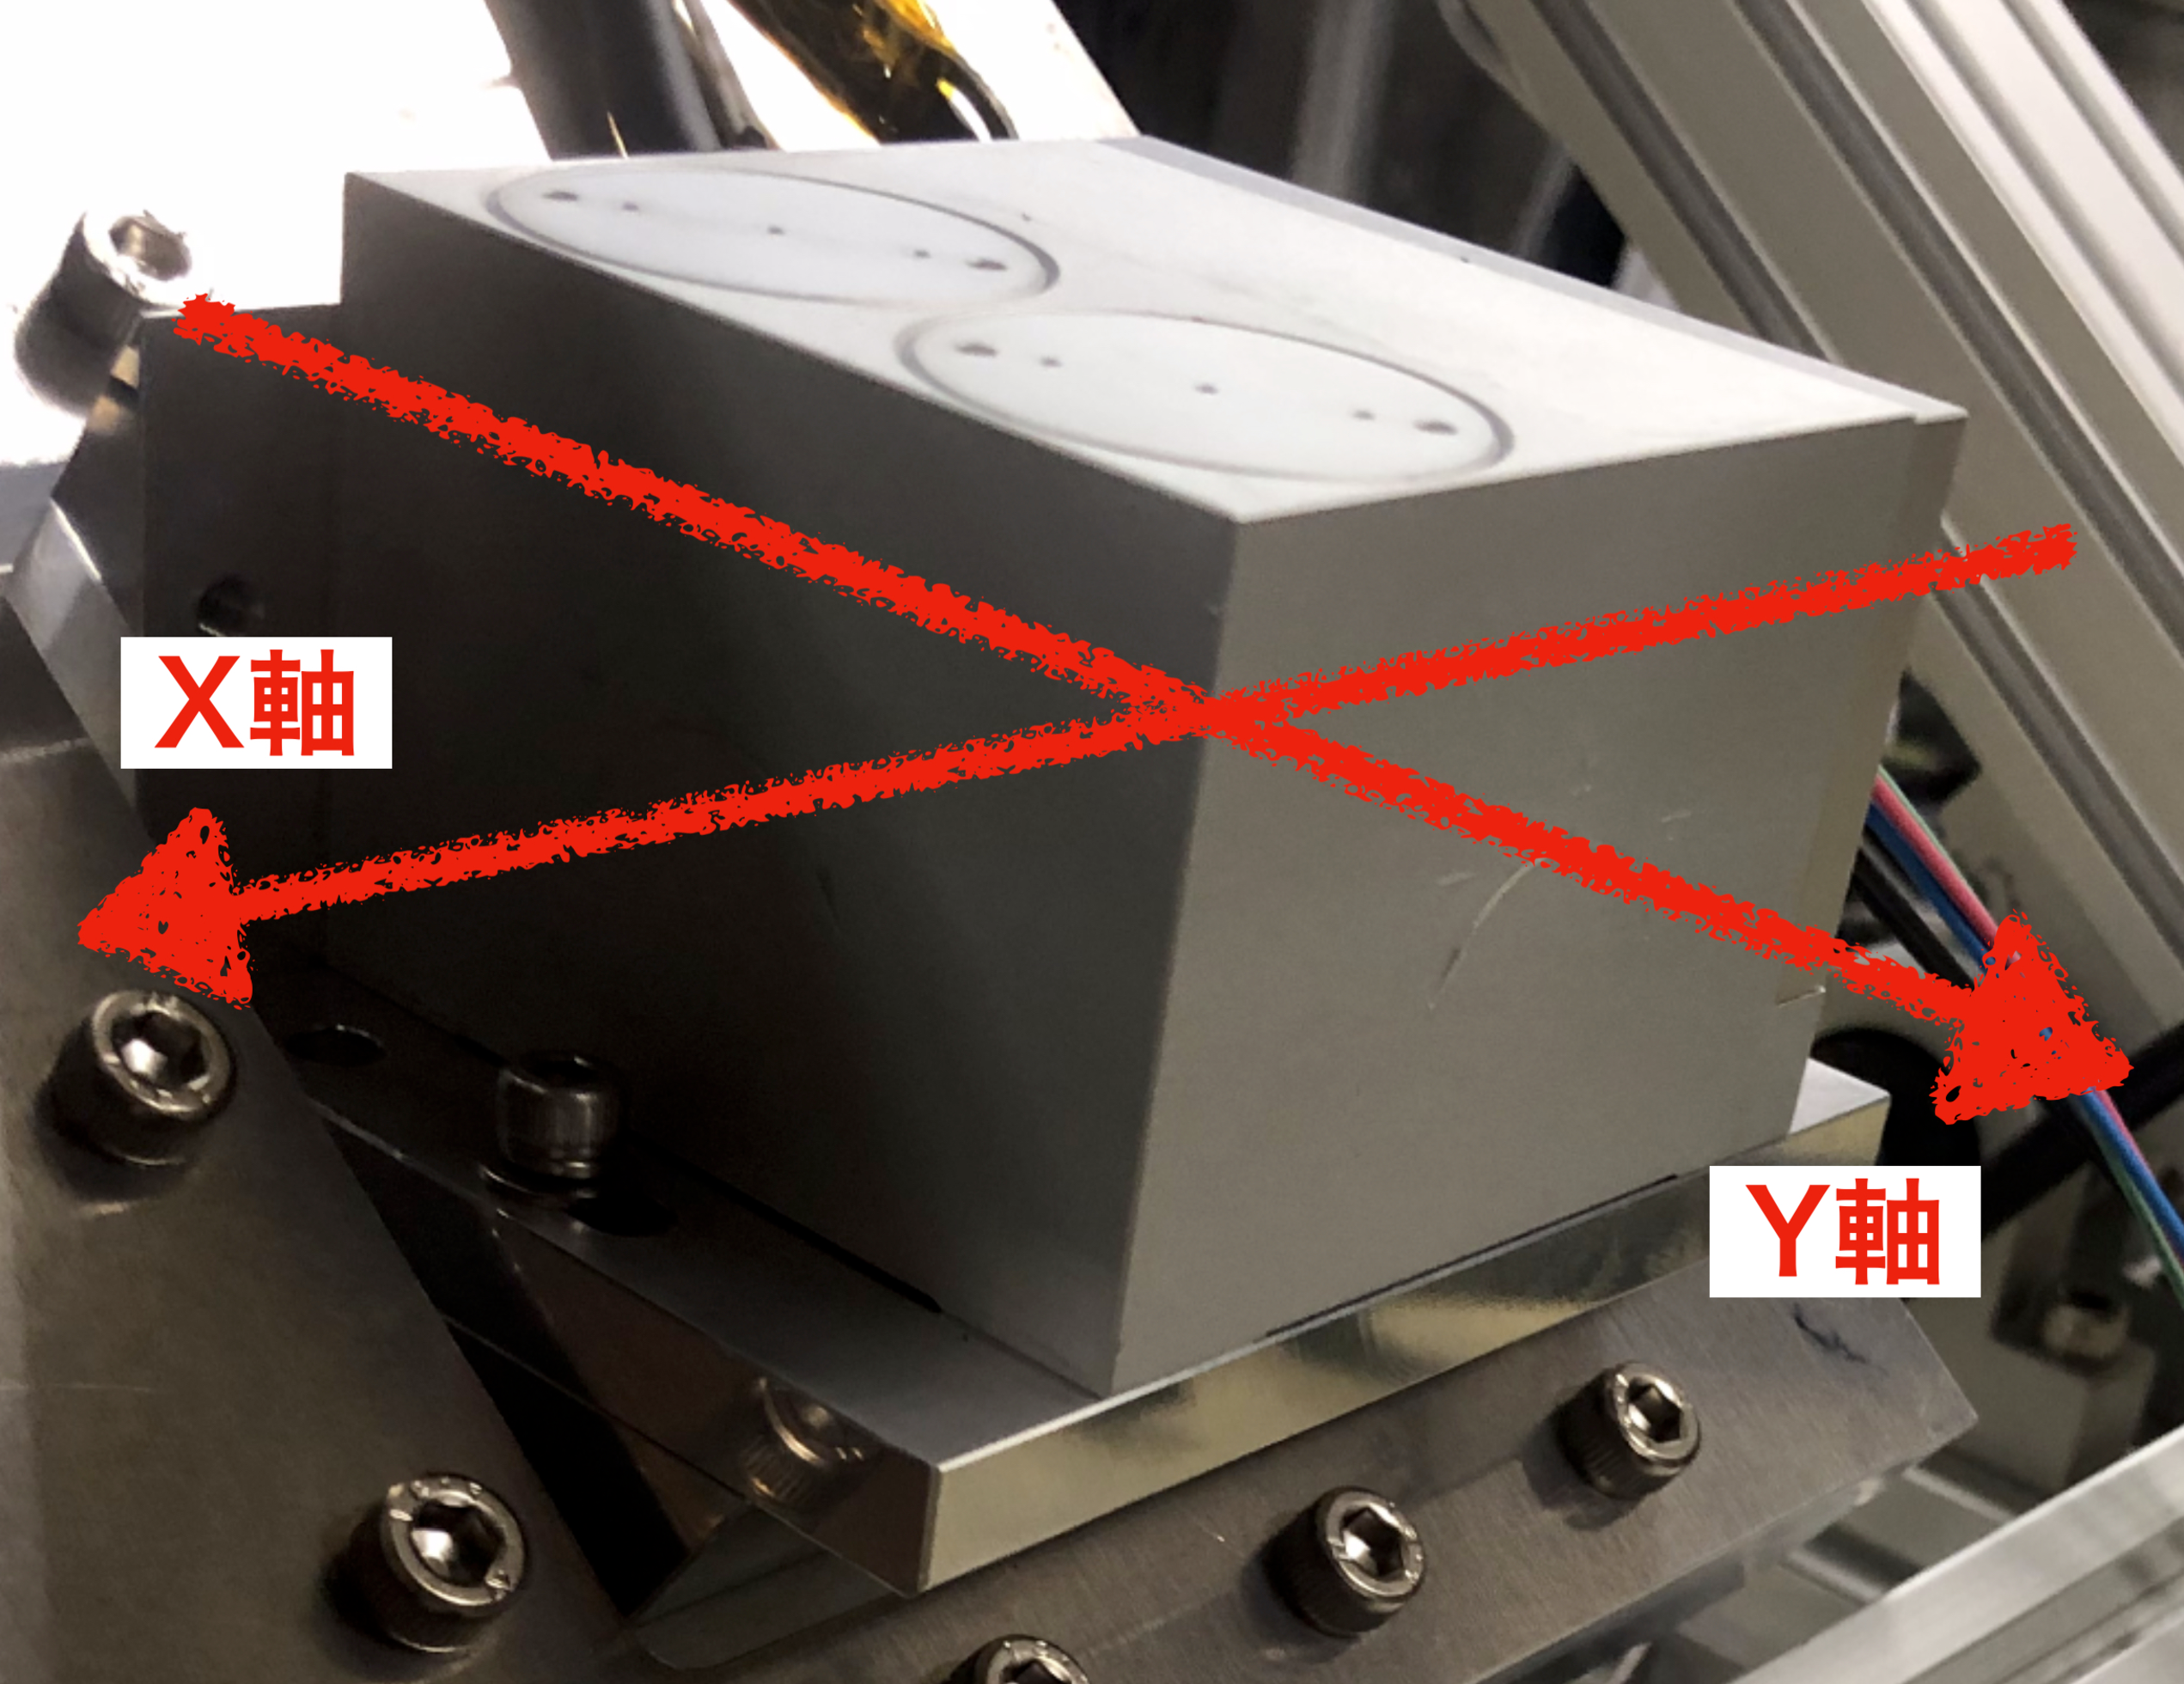
\includegraphics[width=0.5\textwidth]{tiltsensor/tiltsensor_overview.pdf}
    \figcaption{重力参照計 Sherborne Sensors 社 DSIC-2051-60 の外観}
    \label{fig:tiltsensor_DSIC-2051-60}
\end{figure}
% \begin{figure}
%     \centering
%     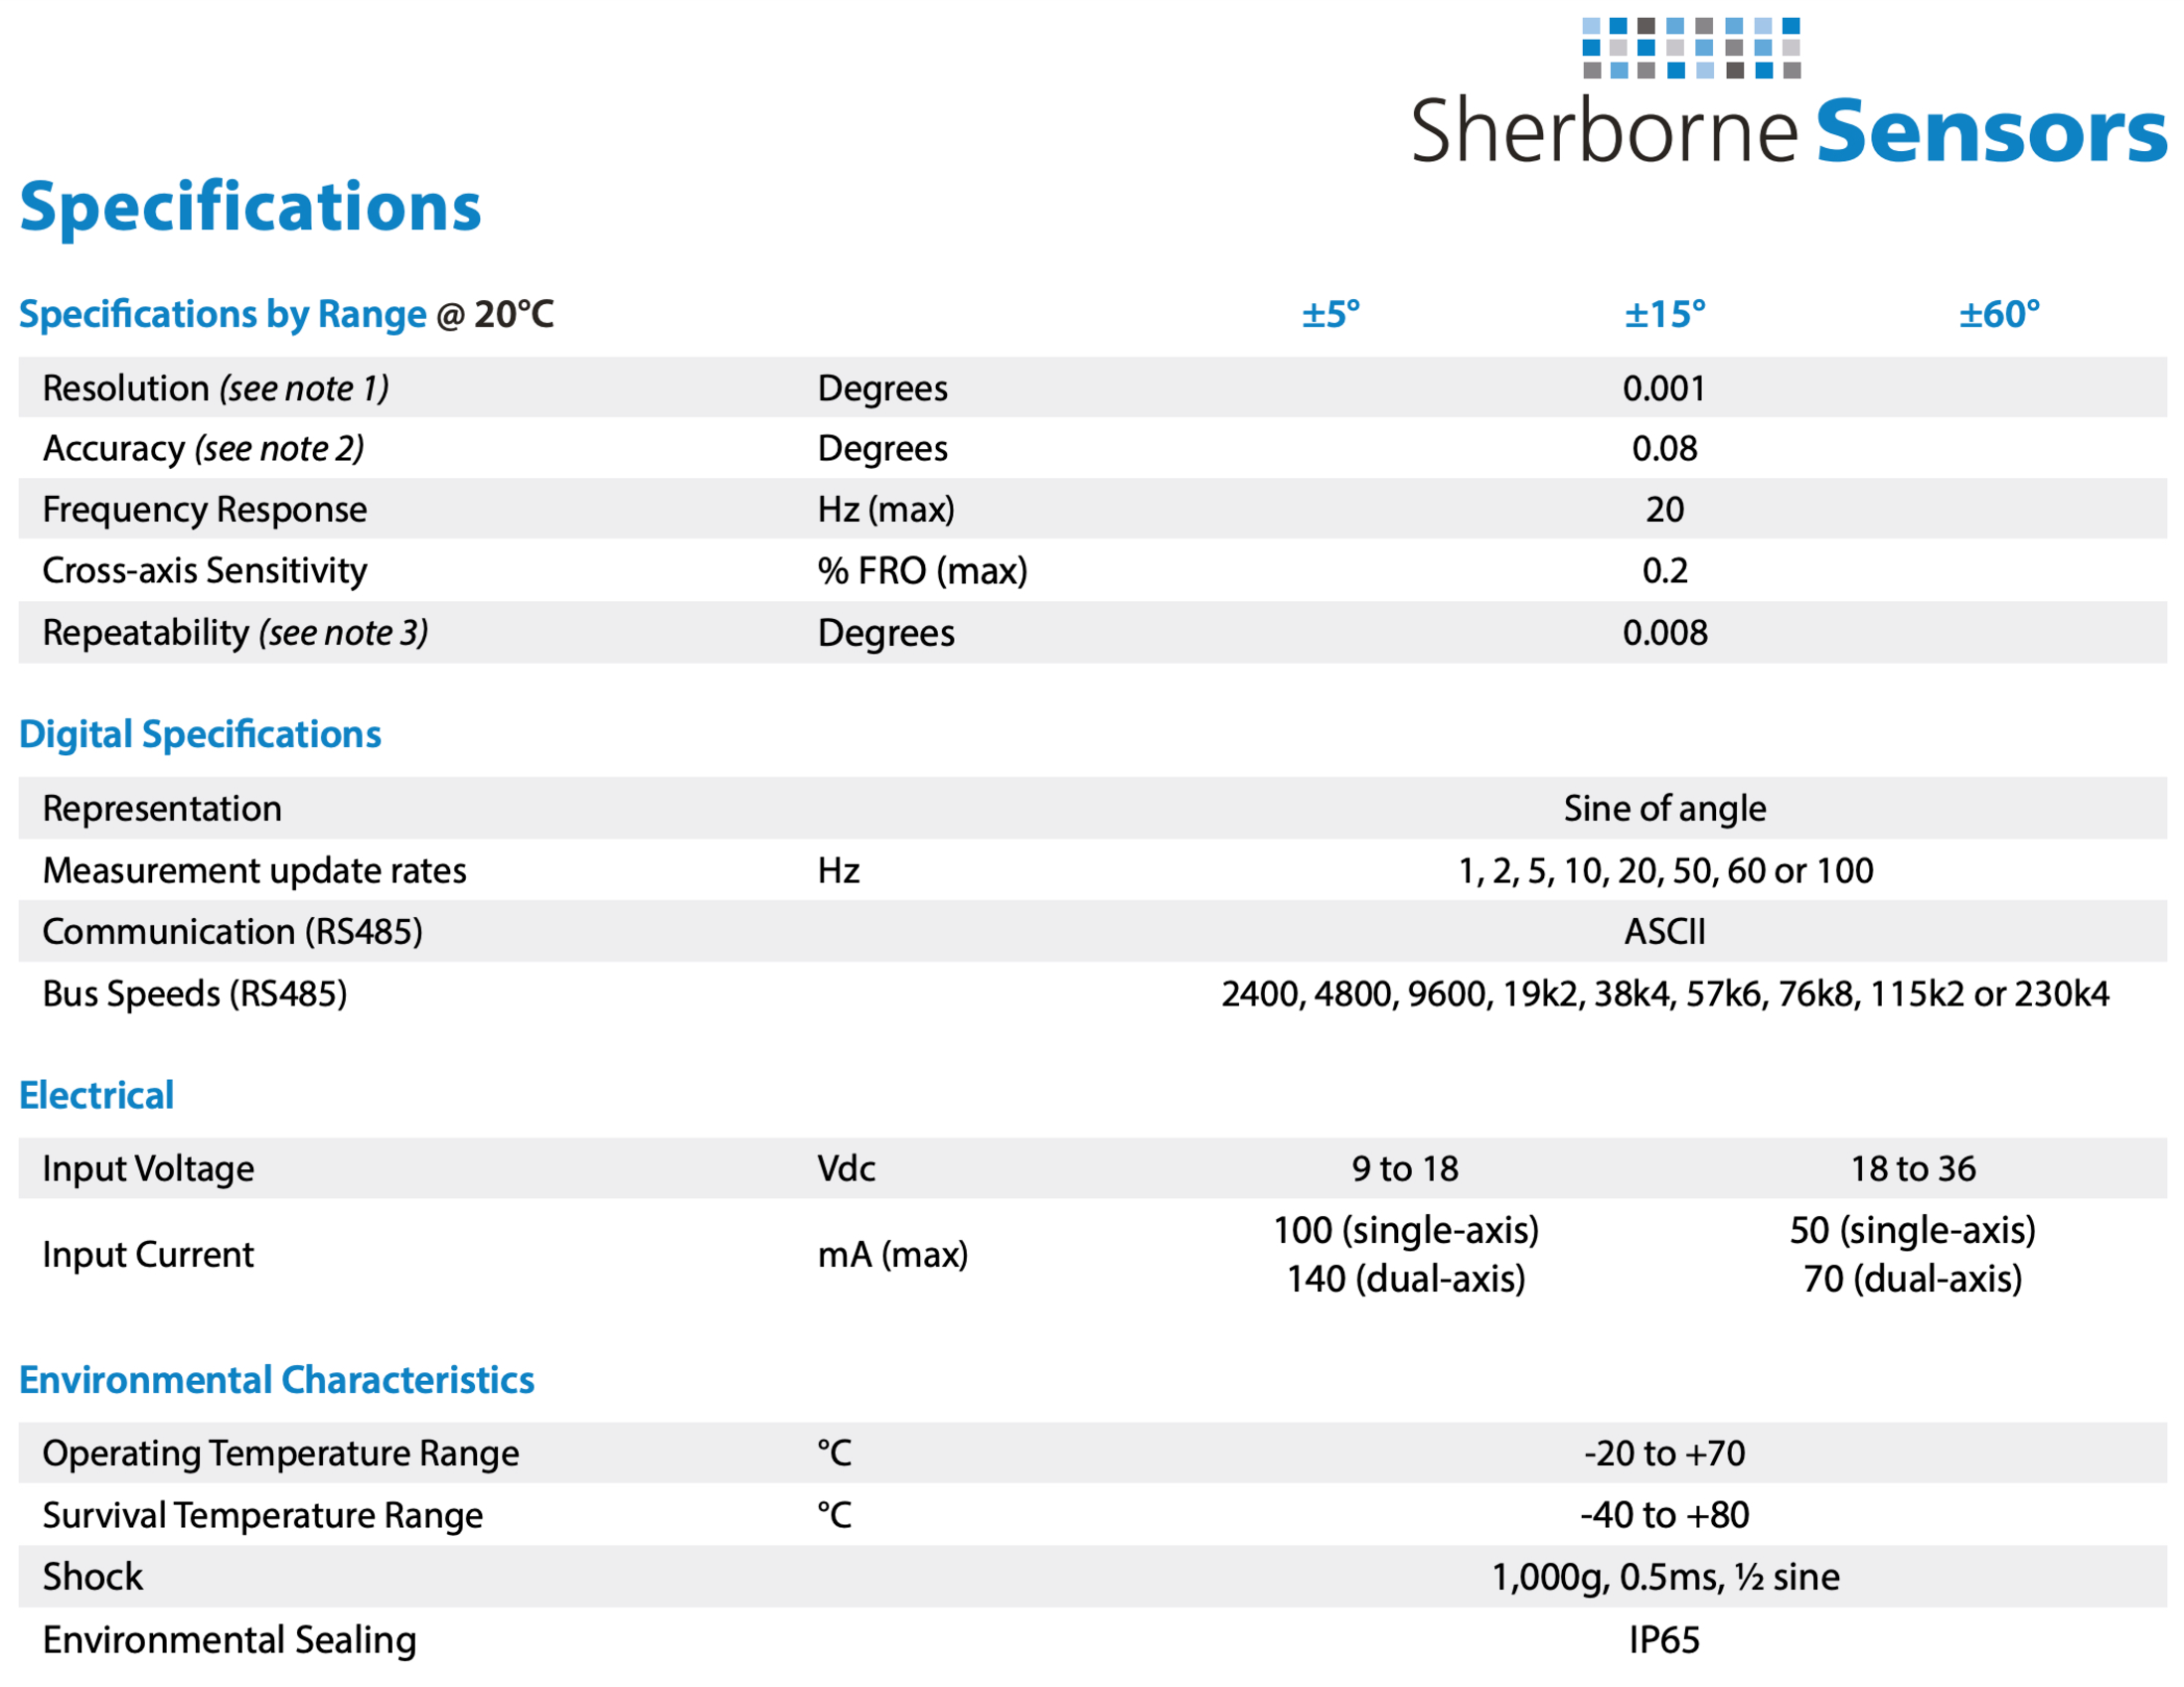
\includegraphics[width=0.5\textwidth]{tiltsensor/sherborne_spec.pdf}
%     \caption{重力参照計 Sherborne Sensors 社 DSIC-2051-60 の仕様}
%     \label{fig:tiltsensor_spec}
% \end{figure}

% \section{電源の入れ直しによるオフセット変動の評価}
% \subsection{評価系}
% 本評価における測定系を図\ref{}に示す。
%水平な机の上に重力参照計を設置した上で、以下の2つの測定を行った。
%\begin{itemize}
%    \item 電源を入れた直後から、10分間データを取得
%    \item 電源を入れた直後100秒待ち、その後30秒間データを取得
%\end{itemize}
%\subsection{測定結果}
%図\ref{}に電源を入れた直後に10分間測定した結果を示す。
\section{温度による出力の変化の評価}
\subsection{評価手法}
図\ref{}に評価系を示す。
重力参照計をアルミニウム製の厚み $\SI{30}{mm}$ のプレートの上に設置した。
このプレートには3つのアジャスターが取り付けられており、これを回すことでプレートの傾きを調整できる。
プレートには新潟精機製の気泡管水準器 FLW-200002 を2つ、互いに垂直になるように設置し、これを参照して
プレート全体が水平になるようにアジャスターで調整した。
この時の水平度の精度は気泡管水準器の精度によって決まり、 $\pm 0.01\tcdegree$ である。
また、プレート上にはUSB温度計を設置し、周囲の空気の温度を測定した。
以上の測定系を恒温槽\footnote{恒温槽は京都市産業技術研究所より拝借した。}に入れ、温度を変化させたときの出力を測定した。

図\ref{fig:bath_temp_usb}にUSB温度計を用いて測定した恒温槽の温度変化の様子を示す。
$\SI{20}{\degreeCelsius}$ から $\SI{-15}{\degreeCelsius}$ まで冷却したのち、再び $\SI{20}{\degreeCelsius}$ まで昇温し、出力の変化を測定した。
各温度 $\SI{10}{\tcdegree}$ 刻みで$\SI{3}{時間}$ ほどかけて変化させ、温度が安定している状態が生まれるようにした。
観測サイトでの気温変動は十分ゆっくりであるか、較正の時間帯を選ぶことで急激な温度変化を避けることができるため、
恒温槽の

\begin{figure}
    \centering
    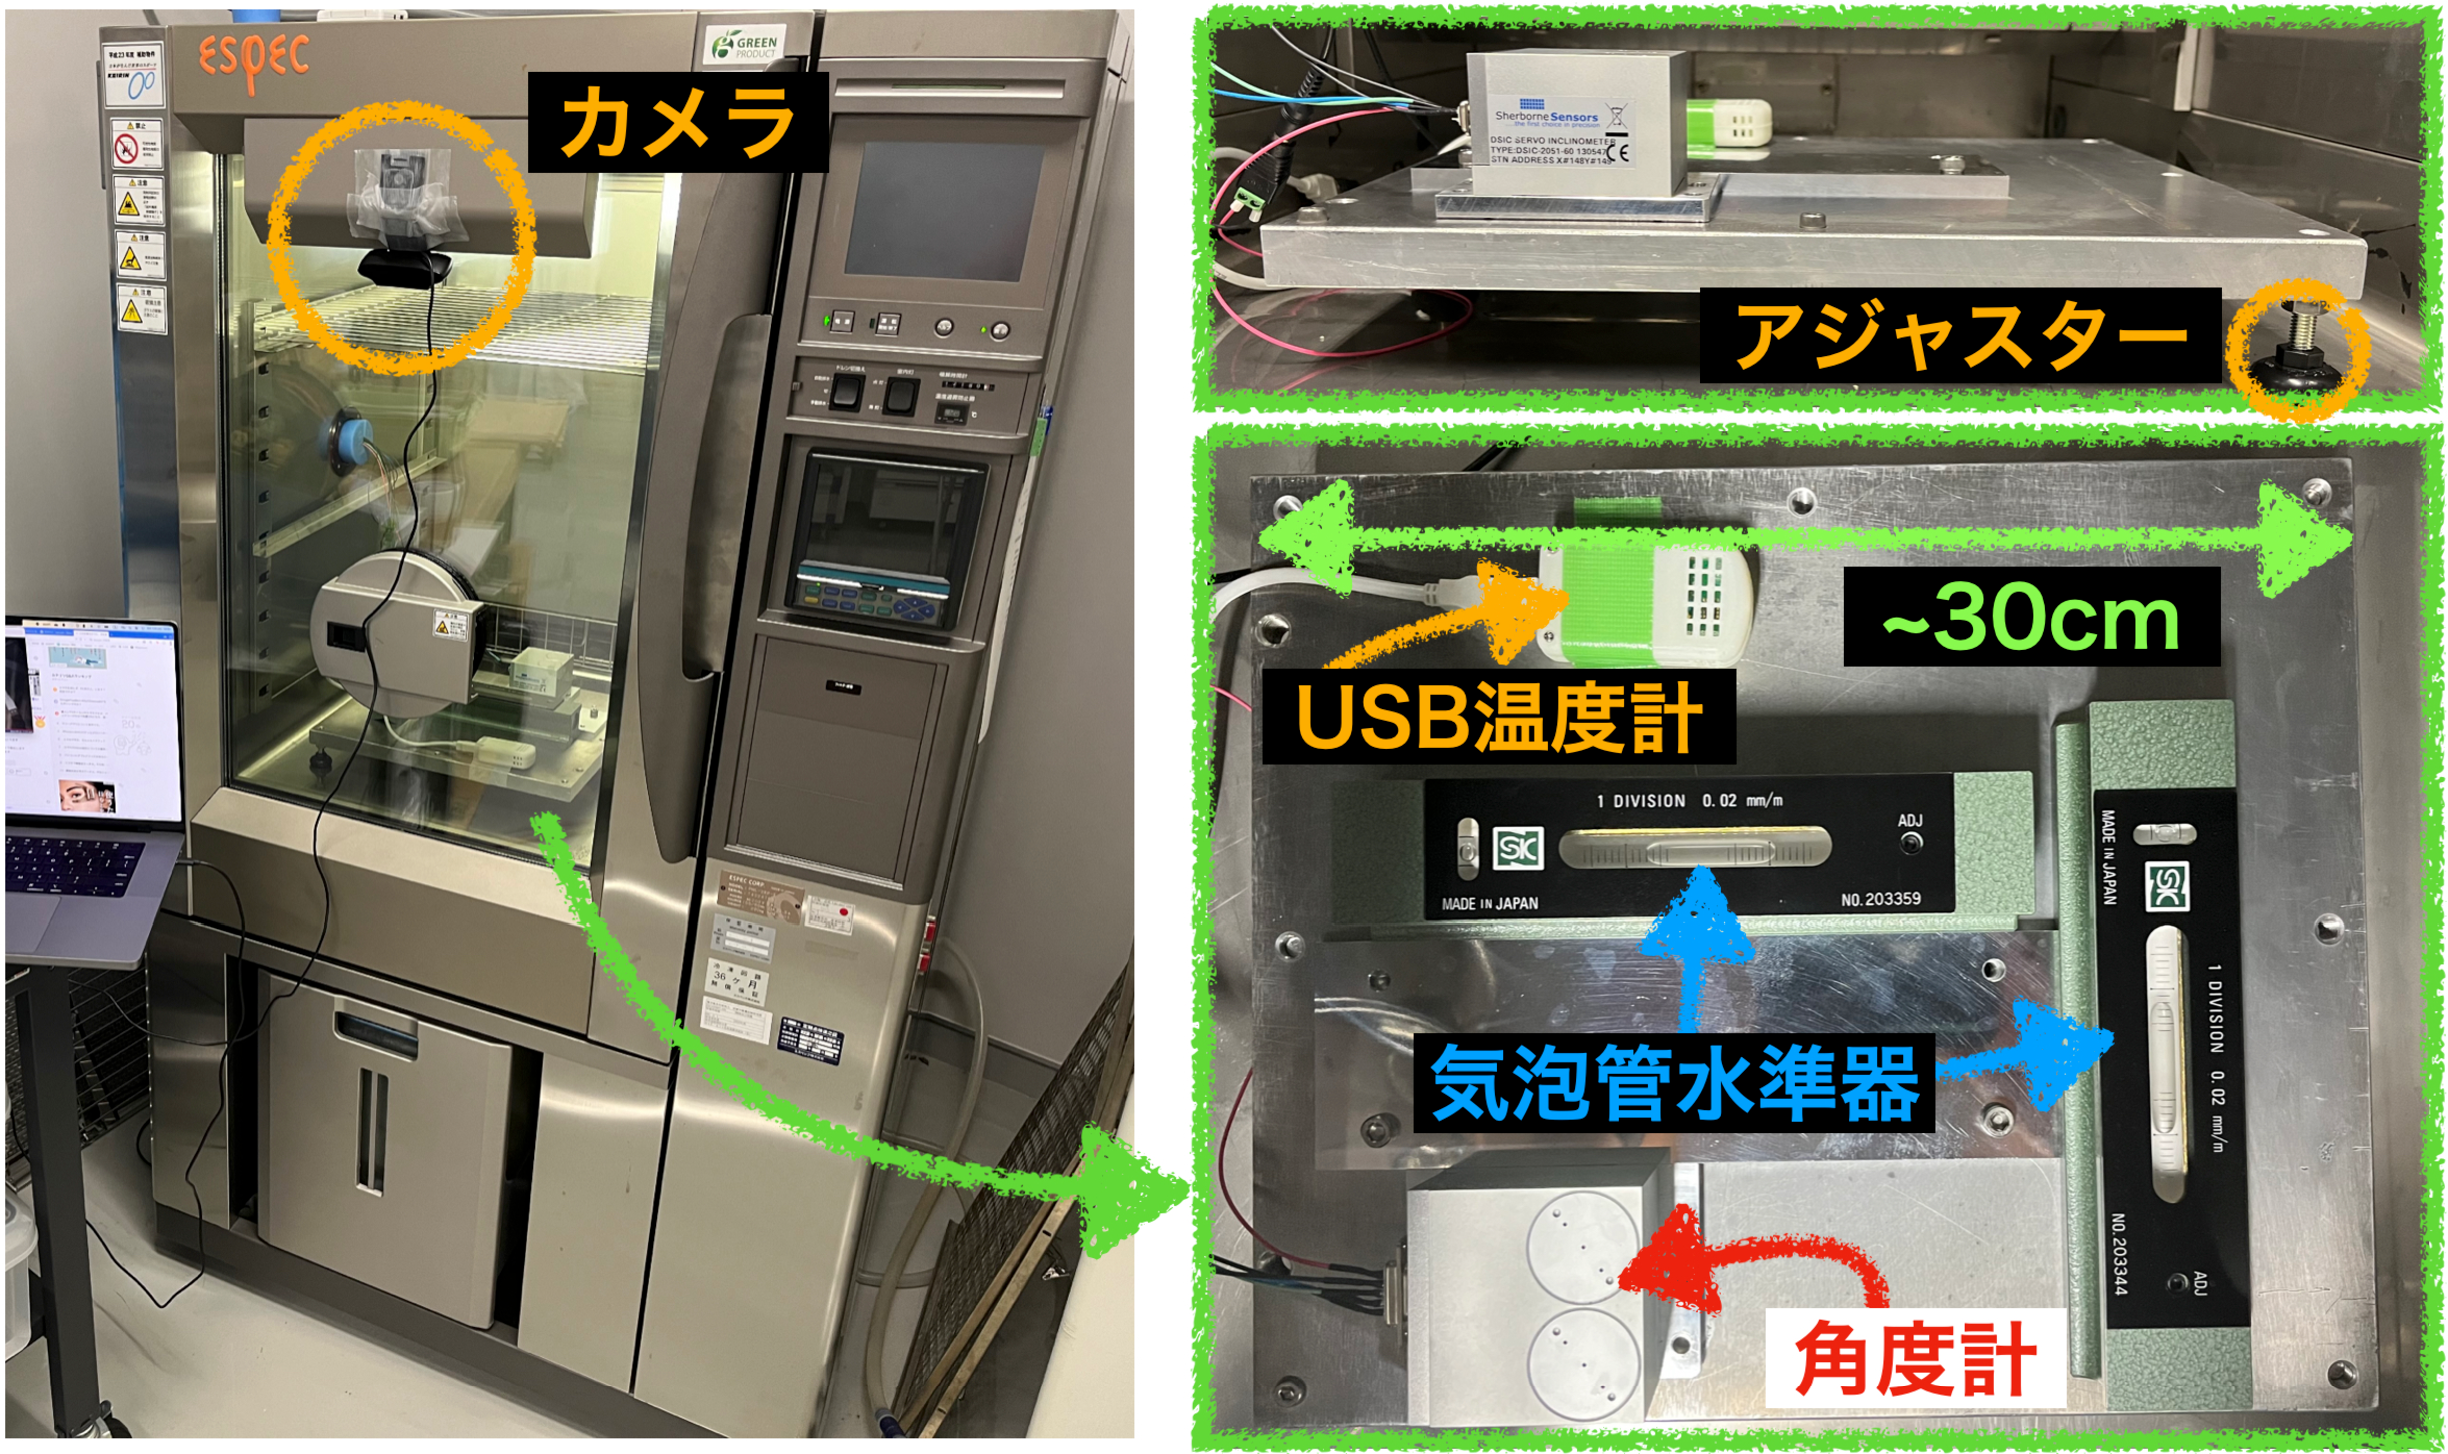
\includegraphics[width=1.0\textwidth]{tiltsensor/evaluation_system.pdf}
    \figcaption{恒温槽を用いた重力参照計の温度変化評価系}
    \label{fig:evaluation_system}
\end{figure}
\begin{figure}[H]
    \centering
    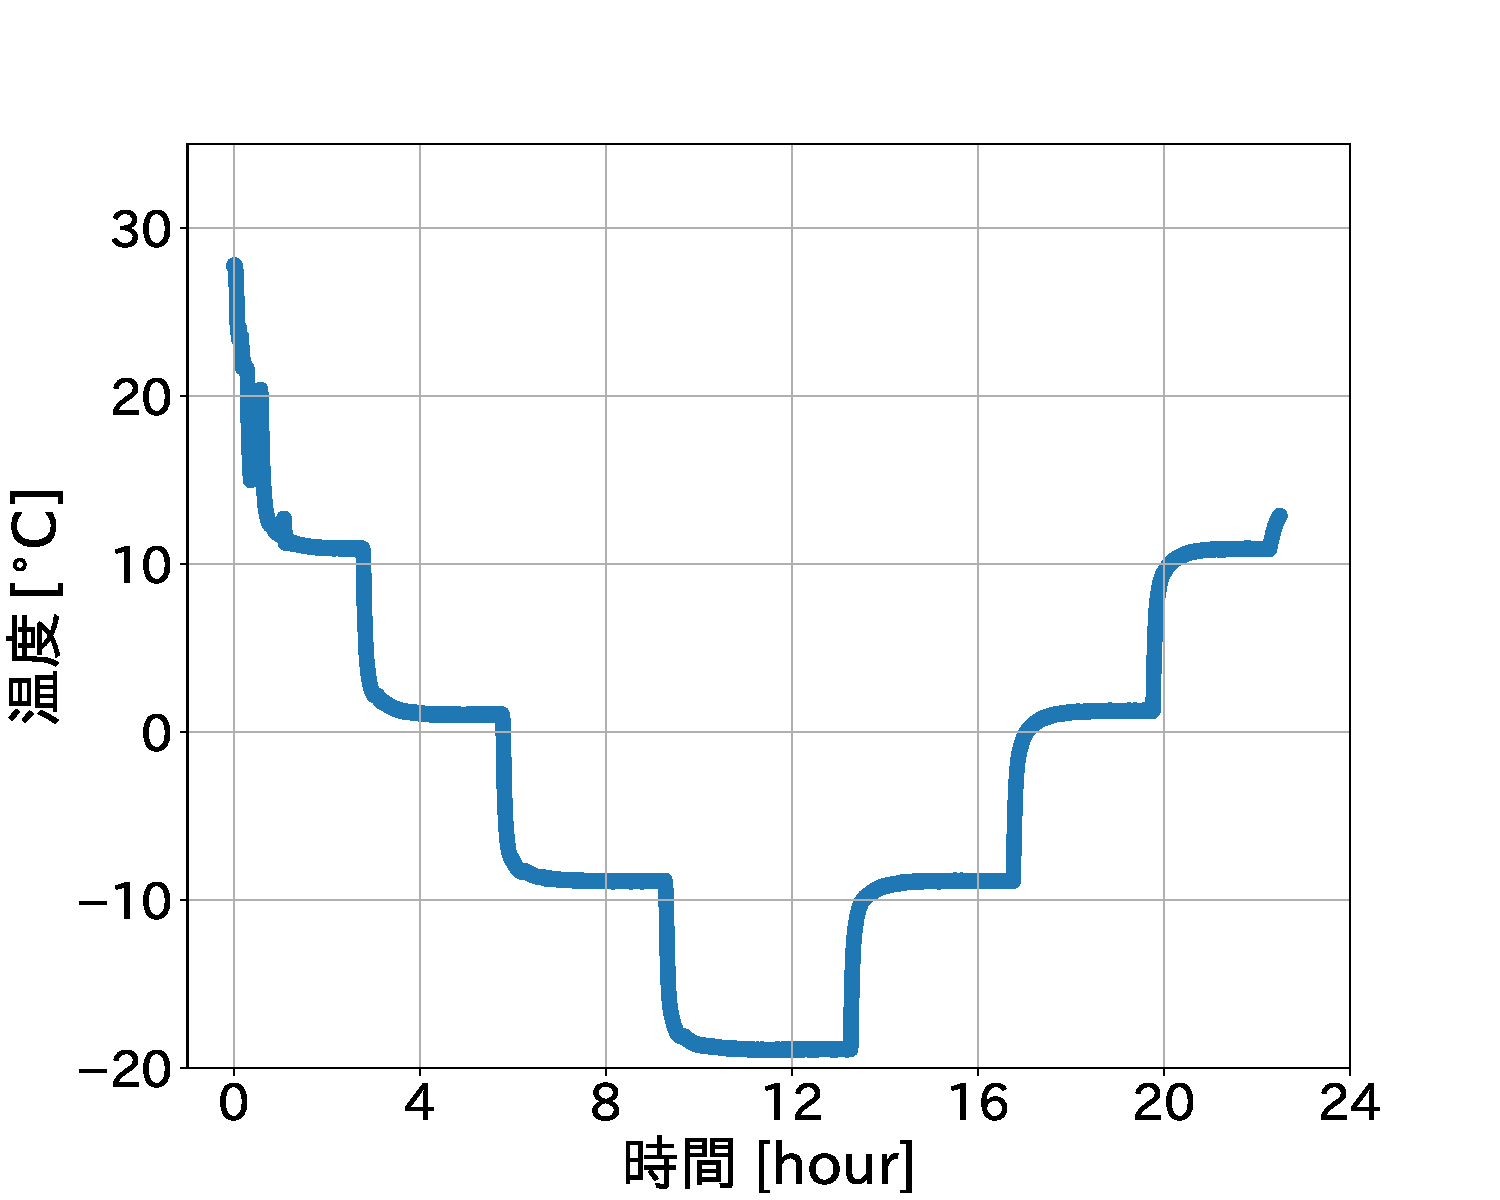
\includegraphics[width=0.8\textwidth]{tiltsensor/bath_temp_usb.pdf}
    \figcaption{恒温槽の温度変化}
    \label{fig:bath_temp_usb}
\end{figure}
\subsection{評価結果}
\subsection{評価結果の考察}
\subsection{まとめ}
\end{document}